\documentclass[12pt,fleqn]{examtst}
\usepackage{graphicx}
\usepackage{amssymb}
\usepackage{amsmath}
\usepackage{listings}
\usepackage{multirow}
\usepackage{multicol}
\usepackage{hhline}
\usepackage{booktabs}
\usepackage{url}
\usepackage{enumerate}
\usepackage{hyperref}
%% Comments

\usepackage{color}

\newif\ifcomments\commentstrue

\ifcomments
\newcommand{\authornote}[3]{\textcolor{#1}{[#3 ---#2]}}
\newcommand{\todo}[1]{\textcolor{red}{[TODO: #1]}}
\else
\newcommand{\authornote}[3]{}
\newcommand{\todo}[1]{}
\fi

\newcommand{\wss}[1]{\authornote{blue}{SS}{#1}}

\begin{document}

\newcommand{\soln}{n} %y for yes and n for no

\lstset{language=python, basicstyle=\ttfamily, breaklines=true,
  showspaces=false, showstringspaces=false, breakatwhitespace=true, texcl=true,
  escapeinside={\%*}{*)}}

\newcommand{\codeit}[1]{\texttt{\textit{#1}}}

\begin{center}
  {\large \bf COMP SCI 2ME3 and SFWR ENG 2AA4 Final Examination}\\[1ex]
  {\large \bf McMaster University}\\[1ex]
  \ifthenelse{\equal{\soln}{y}}{\large {\bf Answer Key:} Large arrow
    ($\Longleftarrow$) for correct% , small ($\leftarrow$) for partially
    % correct
  }{}
\end{center}

\medskip

\noindent
DAY CLASS, \textbf{Version 1}  \hfill Dr.~S.~Smith \\
DURATION OF EXAMINATION: 2.5 hours (+ 30 minutes buffer time)\\
MCMASTER UNIVERSITY FINAL EXAMINATION \hfill April 28, 2021

\medskip

\noindent
\rule[3 mm]{\textwidth}{0.5mm}

%\begin{minipage}[t]{1.0\textwidth}

NAME: \wss{Enter your name here}\\[1ex]

Student ID: \wss{Enter your student number here} \\[2mm]

\noindent
\rule[3 mm]{\textwidth}{0.5mm}

This examination paper includes \noofpages pages and
8 % VARIABILITY
questions. You are responsible for ensuring that your copy of the examination
paper is complete. Bring any discrepancy to the attention
of your instructor.\\

\noindent
\emph{By submitting this work, I certify that the work represents solely my own
independent efforts. I confirm that I am expected to exhibit honesty and use
ethical behaviour in all aspects of the learning process.  I confirm that it is
my responsibility to understand what constitutes academic dishonesty under the
\href{https://secretariat.mcmaster.ca/app/uploads/Academic-Integrity-Policy-1-1.pdf}
{Academic Integrity Policy}}.\\

\noindent
\textbf{Special Instructions}:

\begin{enumerate}

\item For taking tests remotely: 
\begin{itemize}
\item Turn off all unnecessary programs, especially Netflix, YouTube, games like
  Xbox or PS4, anything that might be downloading or streaming.
\item If your house is shared, ask others to refrain from doing those activities
  during the test.
\item If you can, connect to the internet via a wired connection.
\item Move close to the Wi-Fi hub in your house. 
\item Restart your computer, 1-2 hours before the exam. A restart can be very
  helpful for several computer hiccups.
\item Use a VPN (Virtual Private Network) since this improves the connection to
  the CAS servers.
\item Commit and push your tex file, compiled pdf file, and code files
  frequently.  As a minimum you should do a commit and push after completing
  each question.
\item Ensure that you push your solution (tex file, pdf file and code files)
  before time expires on the test.  The solution that is in the repo at the
  deadline is the solution that will be graded.
\item If you have trouble with your git repo, the quickest solution may be to
  create a fresh clone.
\end{itemize}
\item It is your responsibility to ensure that the answer sheet is properly
  completed. Your examination result depends upon proper attention to the
  instructions.
\item All physical external resources are permitted, including textbooks, calculators,
  computers, compilers, and the internet.
\item The work has to be completed individually.  Discussion with others is
  strictly prohibited.
\item Read each question carefully.
\item Try to allocate your time sensibly and divide it appropriately between the
  questions.  Use the allocated marks as a guide on how to divide your time
  between questions.
\item The quality of written answers will be considered during grading.  Please
  make your answers well-written and succinct.
\item The set $\mathbb{N}$ is assumed to include $0$.
\end{enumerate}
%\end{minipage}\\

\examheader{CS2ME3/SE2AA4 \ifthenelse{\equal{\soln}{y}} {\hfill SOLUTIONS} }

\renewcommand{\labelenumi}{\Alph{enumi}.}

\newpage

%%%%%%%%%%%%%%%%%%%%%%%%%%%%%%%%%%%%%%%%%%%%%%%%%%%%%%%%%%%%%%%%%%%%%%

\question{5 marks} What are the problems with using ``average lines of code
written per day'' as a metric for programmer productivity?

\bigskip

\noindent \wss{Provide your reasons in the itemized list below.  Add more items
  as required.}

\begin{itemize}
\item Productivity when it comes to the software development process is a measure of how efficiently the process produces software. However, it is important to note that efficiency does not directly correlate to the number of lines of code written by the developer. There are points in time in the development process where writing an abundance of lines of code is actually frowned upon. In terms of core software qualities, writting more lines of code than necessary often sacrifies essentiality, as there will be times in which lines of code that are not necessarily needed could have been omitted. Additionally, when it comes to writting test cases, it is not necessarily about the number of test cases that are written, but rather how significant the test cases written are for testing all boundaries of the code. This is the key principle of white box testing, where time must be taken to develop test cases that are as close to 100 percent code coverage as possible through specific coverage testing. However, this has nothing to do with the number of lines of code that is written for these test cases, but rather the amount of boundaries and edge cases that the written test cases actually cover. Finally, if a developer is caught up on the number of lines of code they must write, they might sacrifice the crucial time required in the early stages of development when establishing requirements and design for a product. Going directly into implementation may end up increasing the amount of time taken as there was no real effort to consider what the actualy problem is, and how it should be solved. Therefore, although productivity is a difficult measure when it comes to software development, it should not be measured by the number of lines a developer writes.
\end{itemize}

%%%%%%%%%%%%%%%%%%%%%%%%%%%%%%%%%%%%%%%%%%%%%%%%%%%%%%%%%%%%%%%%%%%%%%

\newpage

\question{5 marks} Critique the following requirements specification
for a new cell phone application, called CellApp.  Use the following criteria
discussed in class for judging the quality of the specification: abstract,
unambiguous, and validatable.  How could you improve the requirements
specification?

\bigskip

``The user shall find CellApp easy to use.''

\bigskip

\noindent \wss{Fill in the itemized list below with your answers.  Leave the
  word in bold at the beginning of each item.}

\begin{itemize}
\item \textbf{Abstract} - This specification is abstract because it sticks to stating that the user finds the CellApp easy to use, but does not state how or why this is the case.
\item \textbf{Unambiguous} - This specifification is ambigious because the word "easy" can be interpreted in many different ways and does not give a clear indication of how the user finds the app.
\item \textbf{Validatable} - Because the specification is ambigious and does not give a proper measurement of how easy the user should find the CellApp, this specification is not validatable. 
\item \textbf{How to improve} - In this case, making the specification unambigious is very important as it will ensure that it can be validatable. This can be done by providing more information on what it means for the user to find the app "easy to use". An example would be "The user can run the CellApp in 4 commands". This will allow the specification to be validatable as well.
\end{itemize}

%%%%%%%%%%%%%%%%%%%%%%%%%%%%%%%%%%

\newpage

\question{5 marks} The following module is proposed for the maze tracing robot
we discussed in class (L20).  This module is a leaf module in the decomposition
by secrets hierarchy.

\begin{description}
\item [Module Name] find\_path
\item [Module Secret] The data structure and algorithm for finding the shortest
  path in a graph.
\end{description}

\noindent \wss{Fill in the answers to the questions below.  For each item you
  should leave the bold question and write your answer directly after it.}

\begin{enumerate}
\item \textbf{Is this module Hardware Hiding, Software Decision Hiding or
    Behaviour Hiding?  Why?}

  - This module would be considered software decision hiding. This is because the data structure and algorithm used to find the shortest path in a graph is a software product that can be implemented generally for any graph related problem, and would not necessarily be specific for this maze tracing robot.

\item \textbf{Is this a good secret?  Why?}

  - This is not a good secret. This is because the secret describes both a data structure AND algorith, however a good secret should be specific to one module. To make it better, both the algorithm and data structure for the shortest path should be separated into two different secrets.

\item \textbf{Does the specification for maze tracing robot require environment
    variables?  If so, which environment variables are needed?}

  - The maze tracing robot specification would benefit from an environment variable in order to store the state of the screen itself, the state of the motor of the robot, the position of the robot, etc. This is because the module may interact with the outside environment specifically for the maze tracing robot example.

\end{enumerate}

%%%%%%%%%%%%%%%%%%%%%%%%%%%%%%%%%%

\newpage

\question{5 marks} Answer the following questions assuming that you are in doing
your final year capstone in a group of 5 students.  Your project is to write a
video game for playing chess, either over the network between two human
opponents, or locally between a human and an Artificial Intelligence (AI)
opponent.

\bigskip

\noindent \wss{Fill in the answers to the questions below.  For each item you
  should leave the bold question and write your answer directly after it.}

\begin{enumerate}
  
\item \textbf{You have 8 months to work on the project.  Keeping in mind that we
  usually need to fake a rational design process, what major milestones and what
  timeline for achieving these milestones do you propose?  You can indicate the
  time a milestone is reached by the number of months from the project's start date.}

  - In order to produce quality software, the rational process described by Parnas will act as a great model for my project. We will think about the requirements that the game would like to have, and overall what type of behvaiours we expect the game to have as well. We will then move on to thinking more specifically about the design itself, and how exactly the problem will be solved, including how the requirements will be satisfied. This will be better documented through the use of an MIS, and should be aimed to be completed within 1 month of starting on the project. Once we've gotten a general, but not necessarily conrete idea of the desired implementation, we will begin to code the solution to the problem. In parallel with coding, we should pay attention to potential test cases in order to verify the behaviour and requirements of the code. These steps will be done incrementally in order to eventually build up the software product. Specifically, it would be good practice to make efforts to verify the code through testing every week or so. It is quite possible that while implementing or verifying the product, we will need to make changes to the intiail design and requirements that were written. This is where the idea of "faking the rational design process" comes into play, where we will modify the previously written MIS over the course of time as we encounter more edge cases and design problems within our code. As referenced by the third question, there will also be efforts to berify the installability of the game by testing on external environments such as VMs. This should not be done at the end of the 8 months, but rather incrementally as well, potentially every 2-3 weeks. By maintaining these steps, we can eventually move on to the final stage and think about how the game will be delivered and how we wish to maintain it going forward, potentially 3-4 weeks prior to the end deadline.
  
\item \textbf{Everything in your process should be verified, including the
    verification.  How might you verify your verification?}

  - Mutation testing would be best for verifying your verification. Test cases will be built by intentionally adding faults. These test cases will be run and that these test cases also pick up on the faults that we've added as well. If the test cases are not sufficient, they will not pick up on the seeded faults that were artificially added.
  
\item \textbf{How do you propose verifying the installability of your game?}

  - In order to verify the installability of the game, it is important that I test the game on different environments. This can either be done by asking other users to test the game on their machine, or to use my own virtual machine. This will ensure that the game is able to run on different machines effectively without any unexpected faults. Additionally, this external testing should not be done at the very end of the 8 months, it is important to test on the virtual machine incrementally as time goes on to avoid facing large issues at the very end of development. 
  
\end{enumerate}

%%%%%%%%%%%%%%%%%%%%%%%%%%%%%%%%%%%%%%%%%%%%%%%%%%%%%%%%%%%%%%%%%%%%%%

\newpage

\question{5 marks} As for the previous question, assume you are doing a final
year capstone project in a group of 5 students.  As above, your project
is to write a video game for playing chess, either over the network between two
human opponents, or locally between a human and an Artificial Intelligence
(AI) opponent.  The questions below focus on verification and testing.

\bigskip

\noindent \wss{Fill in the answers to the questions below.  For each item you
  should leave the bold question and right your answer directly after it.}

\begin{enumerate}
\item \textbf{Assume you have 4 work weeks (a work week is 5 days) over the
    course of the project for verification activities.  How many collective
    hours do you estimate that your team has available for verification related
    activities?  Please justify your answer.}

  - Verification of the code is just as important as the implementation itself, because it does not only ensure that the output of the product is the expected/desired result, it also uncovers potential mistakes in both the implementation and indirectly, the initial requirements and design process and allows for an increase in building confidence in the software. It is important that verification is not simply left to the end, but rather integrated throughout the implementation process. For this reason, in accordance with best practices in production environments, it would be my best interest to dedicate 2-3 hours at the end of every work week for such verification activities that involve the entire group, potentially increasing this number as the project becomes more intensive and more code has been written. There should also be individual efforts for verification independent of the team that would also increase this time. Therefore, an estimation of about 20 hours total would be reasonable for verification activities.
  
\item \textbf{Given the estimated hours available for verification, what verification
    techniques do you recommend for your team?  Please list the techniques,
    along with the number of hours your team will spend on each technique, and
    the reason for selecting this technique.}

  - Verification techniques can include analysis, inspection and testing of the software product written. There should be both static and dynamic attempts to verify the software product. First, static techniques such as Rubber Duck testing and code walkthroughs can be used. This includes either the developer sitting by themselves, reading the lines of code to ensure that all lines work as desired, as well as getting in a group environment and talking about the lines of code. This will easily uncover basic faults in the code just be vocalizing the process of the product. Additionally, dynamic testing should be conducted, that involves test cases that are designed specifically for the software product. Although dynamic testing does not guarentee correctness, these tests will still uncover many errors and build confidence in the software. Techniques described by both white-box testing specifically for the code, and black-box testing specifically for the created requirements. The static testing individually, along with the individual test cases run will account for about one third of the 20 allocated hours. The rest will be allocated to more group-based verification techniques, both through more intensive dynamic testing and the code walkthroughs.
  
\item \textbf{Is the oracle problem a concern for implementing your game?  Why
    or why not?  If it is a concern, how do you recommend testing your software?}

  - For a game that we are developing from scratch, chances are there will be components of the expected output/behaviour that is not necessarily known, especially when components of AI technology are desired to be integrated. In this case, oracles will be requierd at each stage of the testing process to tell us what the right answer is, but an oracle itself does not necessarily have to be used. Instead, metamorphic testing will come in handy where an independent program will be used to approximate the oracle. We will manufacture solutions in order to continue on our development process by examining properties of the expected values to determine whether the output itself is wrong. This can be done in addition to previously explained whitebox and blackbox testing.
    
\end{enumerate}

%%%%%%%%%%%%%%%%%%%%%%%%%%%%%%%%%%%%%%%%%%%%%%%%%%%%%%%%%%%%%%%%%%%%%%

\newpage

\question{5 marks} Consider the following natural language specification for a
function that looks for resonance when the input matches an integer multiple of
the wavelengths 5 and 7. Provided an integer input between 1 and 1000, the
function returns a string as specified below:

\begin{itemize}
\item If the number is a multiple of 5, then the output is “resonance 5”
\item If the number is a multiple of 7, then the output is “resonance 7”
\item If the number is a multiple of both 5 and 7, then the output is “resonance
  5 and 7”
\item Otherwise, the output is “no resonance”
\end{itemize}

You can assume that inputs outside of the range 1 to 1000 do not occur.

\begin{enumerate}
\item What are the sets $D_i$ that partition $D$ (the input domain) into a
  reasonable set of equivalence classes?

  - There would need to be 4 sets created in order to cover all of the input domain, while ensuring that all sets are disjoint. The first set would be all integers from 1 to 1000 that are a multiple of 5. The next set would be all integers from 1 to 1000 that are a multiple of 7. The next set would be all integers that are multiples of both 5 and 7. The final set would be all integers that are multiples of neither 5 or 7.

\item Given the sets $D_i$, and the heuristics discussed in class, how would you
  go about selecting test cases?

  - Test cases can be chosen based on the sets created, where suitable test cases must be created for each set. These test cases would be created in accordance to the whitebox coverage testing. In order to achieve both statement and condition coverage, there must be a test case that invokes each of the 4 return statements. There should be additional testing to pay attention to edge coverage. I would draw out a control graph to view all possible routes that the path can be taken, and all possible values of the consituents of compound conditions will be exercised at least once. For example, for the part of the code that should output resonance 5, there should be a case where the number isn't a multiple of 5, and there should be a case for when there is a number of multiple of 5. Many of the cases already created to satisfy the conditions of other parts of the code will already cover part of the edge coverage tests, and so I should make an effort to ensure that there aren't any repeats of tests. Overall, this should include cases in which the value themselves are chosen, values that are very close to 5 and 7, as well as extreme edge cases. This will ideally improve the robustness of the code to test as many cases as possible that are considered to be unexpected.
  
\end{enumerate}
  
%%%%%%%%%%%%%%%%%%%%%%%%%%%%%%%%%%

\newpage

\question{5 marks} Below is a partial specification for an MIS for the game of
tic-tac-toe (\url{https://en.wikipedia.org/wiki/Tic-tac-toe}).  You should
complete the specification.

\bigskip

\wss{The parts that you need to fill in are marked by comments, like this one.
  You can use the given local functions to complete the missing specifications.
  You should not have to add any new local functions, but you can if you feel it
  is necessary for your solution.  As you edit the tex source, please leave the
  \texttt{wss} comments in the file.  You can put your answer immediately
  following the comment.}

\subsection* {Syntax}

\subsubsection* {Exported Constants}

SIZE = 3 {\it //size of the board in each direction}\\

\subsubsection* {Exported Types}

cellT = \{ X, O, FREE \} \\

\subsubsection* {Exported Access Programs}

\begin{tabular}{| l | l | l | p{7cm} |}
\hline
\textbf{Routine name} & \textbf{In} & \textbf{Out} & \textbf{Exceptions}\\
\hline
init & ~ & ~ & ~\\
\hline
move & $\mathbb{N}$, $\mathbb{N}$ & ~ & OutOfBoundsException, InvalidMoveException\\
\hline
getb & $\mathbb{N}$, $\mathbb{N}$ & cellT & OutOfBoundsException\\
\hline
get\_turn & ~ & cellT & ~\\
\hline
is\_valid\_move & $\mathbb{N}$, $\mathbb{N}$ & $\mathbb{B}$ & OutOfBoundsException\\
\hline
is\_winner & cellT & $\mathbb{B}$ & ~\\
\hline
is\_game\_over & ~ & $\mathbb{B}$ & ~\\
\hline

\end{tabular}

\subsection* {Semantics}

\subsubsection* {State Variables}

$b$: boardT\\
$\mathit{Xturn}$: $\mathbb{B}$

\subsubsection* {State Invariant}

\wss{Place your state invariant or invariants here}\\

$\text{number of Xs} + \text{number of Os} + \text{number of FREEs} = 9$ \newline
$\forall i, j \in \mathbb{N}$ such that $b[i][j]$ is a valid cell,$ 0 \le i, j \le 2$

\subsubsection* {Assumptions}

The init method is called for the abstract object before any other access routine is called for that
object.  The init method can be used to return the state of the game to the state of a new game.

\subsubsection* {Access Routine Semantics}

init():
\begin{itemize}
\item transition: 
$$\mathit{Xturn}, b := \text{true}, 
< \begin{array}{c}
< \mbox{FREE}, \mbox{FREE}, \mbox{FREE} >\\
< \mbox{FREE}, \mbox{FREE}, \mbox{FREE} >\\
< \mbox{FREE}, \mbox{FREE}, \mbox{FREE} >\\
\end{array} >
$$
\item exception: none
\end{itemize}

\noindent move($i$, $j$):
\begin{itemize}
\item transition: $\mathit{Xturn}, b[i, j] := \neg \mathit{Xturn}, (\mathit{Xturn} \Rightarrow \mbox{X} | \neg
\mathit{Xturn} \Rightarrow \mbox{O})$
\item exception
$$exc := (\mbox{InvalidPosition}(i, j) \Rightarrow \mbox{OutOfBoundsException} | \neg \mbox{is\_valid\_move}(i, j)
\Rightarrow \mbox{InvalidMoveException})$$
\end{itemize}

\noindent getb(i, j):
\begin{itemize}
\item output: $\mathit{out} := b[i, j]$
\item exception
$exc := (\mbox{InvalidPosition}(i, j) \Rightarrow \mbox{OutOfBoundsException})$
\end{itemize}

\noindent get\_turn():
\begin{itemize}
\item output: $\mathit{Xturn} \Rightarrow \mbox{X} | \neg
\mathit{Xturn} \Rightarrow \mbox{O}$

\item exception: none
\end{itemize}

\noindent is\_valid\_move(i, j):
\begin{itemize}
\item output: $\mathit{out} := (b[i][j] = \mbox{FREE})$ 
\item exception $exc := (\mbox{InvalidPosition}(i, j) \Rightarrow \mbox{OutOfBoundsException})$
\end{itemize}

\noindent is\_winner(c):
\begin{itemize}
\item output: $\mathit{out} := \mbox{horizontal\_win}(c, b) \vee \mbox{vertical\_win}(c, b) \vee
\mbox{diagonal\_win}(c, b)$ 
\item exception: none
\end{itemize}

\noindent is\_game\_over():
\begin{itemize}
\item output: $\mathit{is\_winner(b)} \lor \forall i \in b | i \neq \mbox{FREE} \Rightarrow \mbox{True} | \mbox{True}
 \Rightarrow \mbox{False}$


\item exception: none
\end{itemize}

\subsubsection* {Local Types}

boardT = sequence [SIZE, SIZE] of cellT

\subsubsection* {Local Functions}

\noindent \textbf{InvalidPosition}: $\mathbb{N}$ $\times$ $\mathbb{N}$ $\rightarrow$ $\mathbb{B}$\\
~\newline
InvalidPosition$(i, j) \equiv \neg ( ( 0 \leq i < \mbox{SIZE} ) \wedge ( 0 \leq j < \mbox{SIZE}))$

~\newline

\noindent \textbf{count}: cellT $\rightarrow$ $\mathbb{N}$\\
~\newline
count$(c) \equiv +(i : \mathbb{N} | 0 \leq i \leq \mbox{SIZE} : +(j : \mathbb{N} | 0 \leq j \leq \mbox{SIZE} \land b[i,j] = c : 1))$
~\newline


~\newline

\noindent \textbf{horizontal\_win} : cellT $\times$ boardT $\rightarrow$ $\mathbb{B}$\\
~\newline
horizontal\_win$(c, b) \equiv \exists (i : \mathbb{N} | 0 \leq i < \mbox{SIZE} : b[i, 0] = b[i, 1] = b[i, 2] = c)$

~\newline

\noindent \textbf{vertical\_win} : cellT $\times$ boardT $\rightarrow$ $\mathbb{B}$\\
~\newline
vertical\_win$(c, b) \equiv \exists (j : \mathbb{N} | 0 \leq j < \mbox{SIZE} : b[0, j] = b[1, j] = b[2, j] = c)$

~\newline

\noindent \textbf{diagonal\_win} : cellT $\times$ boardT $\rightarrow$ $\mathbb{B}$\\
~\newline
diagonal\_win$(c, b) \equiv (b[0,0] = b[1,1] = b[2,2] = c) \lor (b[2,0] = b[1,1] = b[0,2] = c)$
~\newline


%%%%%%%%%%%%%%%%%%%%%%%%%%%%%%%%%%

\newpage

\question{5 marks} For this question you will implement in Java an ADT for a 1D
sequence of real numbers.  We want to take the mean of the numbers in the
sequence, but as the following web-page shows, there are several different
algorithms for doing this: \url{https://en.wikipedia.org/wiki/Generalized_mean}

Given that there are different options, we will use the strategy design pattern,
as illustrated in the following UML diagram:

\begin{figure}[!h]
\begin{center}
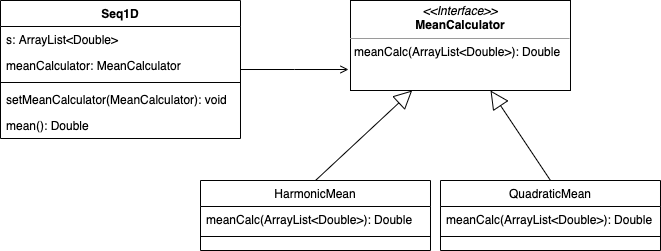
\includegraphics[scale=0.7]{Seq1D_Mean_Strategy_UML.png}
\end{center}
\caption{UML Class Diagram for Seq1D with Mean Function, using Strategy
  Pattern} \label{Fig_UML_Strategy}
\end{figure}

You will need to fill in the following blank files:
\texttt{MeanCalculator.java}, \texttt{HarmonicMean.java},
\texttt{QuadraticMean.java}, and \texttt{Seq1D.java}.  Two testing files are
also provided: \texttt{Expt.java} and \texttt{TestSeq1D.java}.  The file
\texttt{Expt.java} is pre-populated with some simple experiments to help you see
the interface in use, and do some initial testing.  You are free to add to this
file to experiment with your work, but the file itself isn't graded.  The
\texttt{TestSeq1D.java} is also not graded.  However, you may want to create
test cases to improve your confidence in your solution.  The stubs of the
necessary files are already available in your \texttt{src} folder.  The code
will automatically be imported into this document when the \texttt{tex} file is
compiled.  You should use the provided Makefile to test your code.  You will NOT
need to modify the Makefile.  The given Makefile will work for \texttt{make
  test}, without errors, from the initial state of your repo.  The \texttt{make
  expt} rule will also work, because all lines of code have been commented out.
Uncomment lines as you complete work on each part of the modules relevant to
those lines in \texttt{Expt.java} file.  As usual, the final test is whether the
code runs on mills.  You do not need to worry about doxygen comments.

Any exceptions in the specification have names identical to the expected Java
exceptions; your code should use exactly the exception names as given in the
spec.

Remember, your code needs to implement the given specification so that the
interface behaves as specified.  This does NOT mean that the local functions
need to all be implemented, or that the types used internally to the spec need
to be implemented exactly as given.  If you do implement any local functions,
please make them private.  The real type in the MIS should be implemented by
\texttt{Double} (capital D) in Java.

\wss{Complete Java code to match the following specification.}

%%%%%%%%%%%%%%%%%%%%%%%%%%%%%%%%%%

\newpage

\section* {Mean Calculator Interface Module}

\subsection*{Interface Module}

MeanCalculator

\subsection* {Uses}

None

\subsection* {Syntax}

\subsubsection* {Exported Constants}

None

\subsubsection* {Exported Types}

None 

\subsubsection* {Exported Access Programs}

\begin{tabular}{| l | l | l | p{5cm} |}
\hline
\textbf{Routine name} & \textbf{In} & \textbf{Out} & \textbf{Exceptions}\\
\hline
meanCalc & seq of $\mathbb{R}$ & $\mathbb{R}$ & ~\\
\hline
\end{tabular}

\subsubsection* {Considerations}

meanCalc calculates the mean (a real value) from a given sequence of reals.
The order of the entries in the sequence does not matter.

%%%%%%%%%%%%%%%%%%%%%%%%%%%%%%%%%%

\newpage

\section* {Harmonic Mean Calculation}

\subsection*{Template Module inherits MeanCalculator}

HarmonicMean

\subsection* {Uses}

MeanCalculator

\subsection* {Syntax}

\subsubsection* {Exported Constants}

None

\subsubsection* {Exported Types}

None 

\subsubsection* {Exported Access Programs}

\begin{tabular}{| l | l | l | p{5cm} |}
\hline
\textbf{Routine name} & \textbf{In} & \textbf{Out} & \textbf{Exceptions}\\
\hline
meanCalc & seq of $\mathbb{R}$ & $\mathbb{R}$ & ~\\
\hline
\end{tabular}

\subsection* {Semantics}

\subsubsection* {State Variables}

None

\subsubsection* {State Invariant}

None

\subsubsection* {Assumptions}

None

\subsubsection* {Access Routine Semantics}

meanCalc($v$)
\begin{itemize}
\item output: $\mathit{out} := \frac{|x|}{+(x: \mathbb{R} | x \in v : 1/x)}$
\item exception: none
\end{itemize}

%%%%%%%%%%%%%%%%%%%%%%%%%%%%%%%%%%

\newpage

\section* {Quadratic Mean Calculation}

\subsection*{Template Module inherits MeanCalculator}

QuadraticMean

\subsection* {Uses}

MeanCalculator

\subsection* {Syntax}

\subsubsection* {Exported Constants}

None

\subsubsection* {Exported Types}

None 

\subsubsection* {Exported Access Programs}

\begin{tabular}{| l | l | l | p{5cm} |}
\hline
\textbf{Routine name} & \textbf{In} & \textbf{Out} & \textbf{Exceptions}\\
\hline
meanCalc & seq of $\mathbb{R}$ & $\mathbb{R}$ & ~\\
\hline
\end{tabular}

\subsection* {Semantics}

\subsubsection* {State Variables}

None

\subsubsection* {State Invariant}

None

\subsubsection* {Assumptions}

None

\subsubsection* {Access Routine Semantics}

meanCalc($v$)
\begin{itemize}
\item output: $\mathit{out} := \sqrt{\frac{+(x: \mathbb{R} | x \in v : x^2)}{|x|}}$
\item exception: none
\end{itemize}

%%%%%%%%%%%%%%%%%%%%%%%%%%%%%%%%%%

\newpage

\section* {Seq1D Module}

\subsection* {Template Module}

Seq1D

\subsection* {Uses}

MeanCalculator

\subsection* {Syntax}

\subsubsection* {Exported Types}

Seq1D = ?

\subsubsection* {Exported Constants}

None

\subsubsection* {Exported Access Programs}

\begin{tabular}{| l | l | l | p{6cm} |}
\hline
\textbf{Routine name} & \textbf{In} & \textbf{Out} & \textbf{Exceptions}\\
\hline
new Seq1D & seq of $\mathbb{R}$, MeanCalculator & Seq1D & IllegalArgumentException\\
\hline
setMaxCalculator & MaxCalculator &  & \\
\hline
mean &  & $\mathbb{R}$ & \\
\hline

\end{tabular}

\subsection* {Semantics}

\subsubsection* {State Variables}

$s$: seq of $\mathbb{R}$\\
meanCalculator: MeanCalculator

\subsubsection* {State Invariant}

None

\subsubsection* {Assumptions}

\begin{itemize}
\item The Seq1D constructor is called for each object instance before any other
  access routine is called for that object.  The constructor can only be called
  once.  All real numbers provided to the constructor will be zero or positive.
\end{itemize}

\subsubsection* {Access Routine Semantics}

new Seq1D($x$, $m$):
\begin{itemize}
\item transition: $s, \text{meanCalculator} := x, m$
\item output: $\mathit{out} := \mathit{self}$
\item exception:
  $\mathit{exc} := (|x| = 0 \Rightarrow \mbox{IllegalArgumentException})$
\end{itemize}

\noindent setMeanCalculator($m$):
\begin{itemize}
\item transition: $\mbox{meanCalculator} := m$
\item exception: none
\end{itemize}

\noindent mean():
\begin{itemize}
\item output: $\mathit{out} := \mbox{meanCalculator.meanCalc}()$
\item exception: none
\end{itemize}

%%%%%%%%%%%%%%%%%%%%%%%%%%%%%%%%%%

\newpage

\subsection*{Code for MeanCalculator.java}

\noindent \lstinputlisting[language = Java]{./src/MeanCalculator.java}

\newpage

\subsection*{Code for HarmonicMean.java}

\noindent \lstinputlisting[language = Java]{./src/HarmonicMean.java}

\newpage

\subsection*{Code for QuadraticMean.java}

\noindent \lstinputlisting[language = Java]{./src/QuadraticMean.java}

\newpage

\subsection*{Code for Seq1D.java}

\noindent \lstinputlisting[language = Java]{./src/Seq1D.java}

%%%%%%%%%%%%%%%%%%%%%%%%%%%%%%%%%%

\end{document}